\documentclass[10pt,oneside]{book}

%%%%%%%%%%%%%%%%%
% import packages %
%%%%%%%%%%%%%%%%%
\usepackage{lipsum}
\usepackage{lmodern}
\usepackage{ragged2e}
\usepackage{adjustbox}
\usepackage{array}
\usepackage{rotating}
\usepackage{array}
\usepackage{setspace}
\usepackage{algorithm}
\usepackage{algpseudocode}
\usepackage{multirow}
\usepackage{booktabs}
\usepackage{makecell}
\usepackage{tcolorbox}
\usepackage{graphicx} 
\usepackage{fancybox} 
\usepackage{soul,color}
\usepackage{amsmath}
\usepackage{pdfpages}
\usepackage{tocloft}
\usepackage{amssymb}
\usepackage{tikz}
\usepackage{titlesec}
\usepackage{titletoc}
\usepackage{tabularx}
\usepackage{hyperref}
\usepackage{epigraph}
\usepackage{pdfpages}
\usepackage{pdflscape}
\usepackage{afterpage}
\usepackage{tablefootnote}
\usepackage{rotating}
\usepackage{pgfgantt}
\usepackage[acronyms]{glossaries}
\usepackage[
layout=letterpaper, 
paper=letterpaper, 
portrait, 
head=0.5in,
foot=0.5in,
top=.75in, 
bottom=.75in, 
left=0.75in, 
right=0.75in, 
margin=1in
]{geometry}
\usepackage[style=numeric-comp,backend=biber,backref=true,sorting=none]{biblatex}
\usepackage{cleveref}
\usepackage[toc,page]{appendix}
\usepackage{subfiles} % best loaded last in the preamble

% Custom column type for ragged-right with a fixed width
\newcolumntype{L}[1]{>{\raggedright\let\newline\\\arraybackslash\hspace{0pt}}m{#1}}

\makeglossaries

%Acronyms
\newacronym{tar}{TAR}{Technology-Assisted Review}
\newacronym{cal}{CAL}{Continuous Active Learning}
\newacronym{llm}{LLM}{Large Language Model}
\newacronym{gnn}{GNN}{Graph Neural Network}
\newacronym{gcn}{GCN}{Graph Convolutional Network}
\newacronym{gats}{GATs}{Graph Attention Networks}
\newacronym{bcs}{BCS}{Backwards Citation Searching}
\newacronym{fcs}{FCS}{Forwards Citation Searching}
\newacronym{ebm}{EBM}{Evidence-Based Medicine}
\newacronym{spl}{SPL}{Simple Passive Learning}
\newacronym{sal}{SAL}{Simple Passive Learning}
\newacronym{rcts}{RCTs}{Randomised Controlled Trials}
\newacronym{ir}{IR}{Information Retrieval}
\newacronym{tfidf}{TF-IDF}{Term Frequency-Inverse Document Frequency}
\newacronym{mlm}{MLM}{Masked Language Modelling}

% %%%%%%%%%%%%%%%%%%%%%%%%%%%%%%%%%%%%%%%%%%
% % Other commands
% %%%%%%%%%%%%%%%%%%%%%%%%%%%%%%%%%%%%%%%%%%

\newcommand{\bibliographyLSR}[1]{\bibliography{#1}}
\newcommand{\ts}{\textsuperscript} %sobrescrito

\onehalfspacing

\AtBeginBibliography{\small}

\usetikzlibrary{shapes, arrows, positioning, fit,backgrounds}
\usetikzlibrary{arrows.meta}

\hypersetup{
colorlinks=true,
urlcolor=blue,
linkcolor=blue,
citecolor=blue,
pdftitle={@title - @author},
pdfsubject={Systematic Review},
pdfauthor={@author},
pdfkeywords={list; here; your; keywords (key words)}
}

\addbibresource{zot_references.bib}
\setlength{\cftsecnumwidth}{2.5em}
\setcounter{tocdepth}{1}
\begin{document}
\section{Systematic reviews}

Systematic reviews provide a rigorous and transparent approach to synthesising research evidence on a specific topic, forming a cornerstone of evidence-based practice. Unlike traditional narrative reviews, systematic reviews adhere to a pre-defined, systematic methodology that minimises bias and ensures reproducibility. This methodical approach encompasses comprehensive literature searches, critical appraisal of studies, and careful synthesis of findings, ultimately providing a reliable and comprehensive overview of the current state of knowledge.

The term \emph{systematic} underscores the methodical and structured approach used throughout the review process. While the precise execution varies depending on the type of review and research question, several core characteristics define this methodology:

\begin{itemize}
    \item {\bf{Explicit, Step-by-Step Methodology:}} systematic reviews follow a clearly defined, step-by-step methodology, often documented in comprehensive procedural manuals. In medicine, for instance, the Cochrane Collaboration's Review Manual \cite{lefebvre_cochrane_2011} provides a detailed guide to conducting Cochrane Reviews. Similarly, in qualitative research, Noblit and Hare's book on meta-ethnography \cite{noblit_meta-ethnography_1988} outlines procedures for synthesising qualitative studies. These manuals provide a framework for standardised, transparent reviews.
    \item {\bf{Pre-Established Review Protocol:}} systematic reviews require the development of a detailed protocol {\it{before}} the review commences. This protocol acts as a blueprint, outlining the review's objectives, search strategy, inclusion and exclusion criteria, data extraction methods, and analysis plan. The pre-defined protocol prevents arbitrary changes in the review's scope during the process and minimises duplication of effort among reviewers. Furthermore, many reviewers register their protocols in publicly accessible registries like PROSPERO\footnote{https://www.crd.york.ac.uk/prospero/}, or open-access platforms, enhancing transparency and accountability \cite{tawfik_protocol_2020}.
    \item {\bf{Reporting Guidelines:}} systematic reviews adhere to established reporting guidelines to ensure clarity and consistency. These guidelines specify the essential elements to include in the final review report \cite{moher_preferred_2010}. Numerous reporting guidelines are available, tailored to various review types and research designs. Resources like the EQUATOR Network\footnote{https://www.equator-network.org/} compile and offer these guidelines, promoting standardised reporting across different fields.
    
    \item {\bf{Quality Assessment Checklist:}} The checklist provides an assessment of the methodological quality (risk of bias) of included studies, aiding the reader in interpreting the overall credibility of the review's findings. This allows the reader to answer the question, ``Is this a good or bad example of a review?". This process typically uses validated quality assessment checklists or tools appropriate for the study designs under review \cite{whiting_proposed_2017}.
    \item {\bf{Methodological Surveys or Audits:}} Methodological surveys or audits evaluate how emerging review types (e.g., scoping or umbrella reviews) are conducted, often signalling the need for refined reporting standards. They can occur before formal guidelines are established or continuously e.g., \cite{dalton_potential_2017, france_methodological_2014}. By aggregating practices from published reviews, they identify methodological inconsistencies (e.g., misuse of meta-analysis for heterogeneous data) or innovations. Such audits signal when a review type gains traction and inform consensus on best practices, often catalysing reporting standards (e.g., PRISMA extensions) or warnings against flawed approaches \cite{tricco_prisma_2018, sarkis-onofre_how_2021,rethlefsen_prisma-s_2021, rethlefsen_prisma-s_2021-1}
\end{itemize}

While this document explores the methodologies and challenges of systematic reviews, its literature review, constrained by the typical limitations of a PhD project, cannot be a full systematic review because systematic reviews are resource-intensive, often requiring dedicated funding, a multi-year timeframe, and a multidisciplinary team.
\subsection{In medicine}

% systematic review use in medicine.
Central to medical research and practice, systematic reviews synthesise existing literature on clearly framed clinical questions \cite{kranke_evidence-based_2010, higgins_cochrane_2019}. They consolidate extensive evidence into a cohesive, critically appraised summary that offers clear decision support for clinicians and policymakers. systematic reviews are created across virtually every medical subspecialty. Recent publications illustrate their scope, exploring cardiovascular risks in endometriosis \cite{parsa_endometriosis_2025}, clarifying links between antidepressants and insomnia in adolescents \cite{turkmen_systematic_2025}, and examining anaemia in pregnancy \cite{azzam_anemia_2025}. The exponential growth of new studies necessitates reliance on systematic syntheses for reliable, up-to-date guidance.


% How systematic reviews support decision making
Systematic reviews provide the highest-ranked evidence for many clinical questions in \gls*{ebm} underpinning clinical decision-making. As shown in Table \ref{tab:evidence_levels}, \gls*{ebm} organises evidence types hierarchically, ranking expert opinion as the weakest (level 5) and systematic reviews of \gls*{rcts} as the strongest (level 1a). To minimise bias, systematic reviews, unlike traditional narrative reviews, follow strict methodological guidelines such as comprehensive literature searches and critical appraisal of each included study. This rigorous approach ensures a transparent and reproducible evidence synthesis, enabling practitioners to make more informed decisions tailored to patient needs.

\begin{table}[ht]
\centering
\small
\begin{adjustbox}{width=\columnwidth/2}
\begin{tabular}{|c|l|}
\hline
\textbf{Level} & \textbf{Type of Evidence} \\
\hline
1a & Systematic reviews of randomised controlled trials \\
1b & Individual randomized controlled trials \\
2a & Systematic reviews of cohort studies \\
2b & Individual cohort studies \\
3a & Systematic reviews of case-control studies \\
3b & Individual case-control studies \\
4 & Case series \\
5 & Expert opinion \\
\hline
\end{tabular}
\end{adjustbox}
\caption[A summarised form of the 2009 OCEBM Levels of Evidence]{A summarised form of the 2009 OCEBM Levels of Evidence \cite{noauthor_oxford_nodate} There are conflicting thoughts on the absolute ranking of strength for all evidence sources \cite{swanson_how_2010, guyatt_grade_2008}; however, a key commonality is that systematic reviews (of \glspl*{rct}) are considered the strongest evidence type.}
\label{tab:evidence_levels}
\end{table}

% Growth of systematic reviews
\begin{figure}
    \centering
    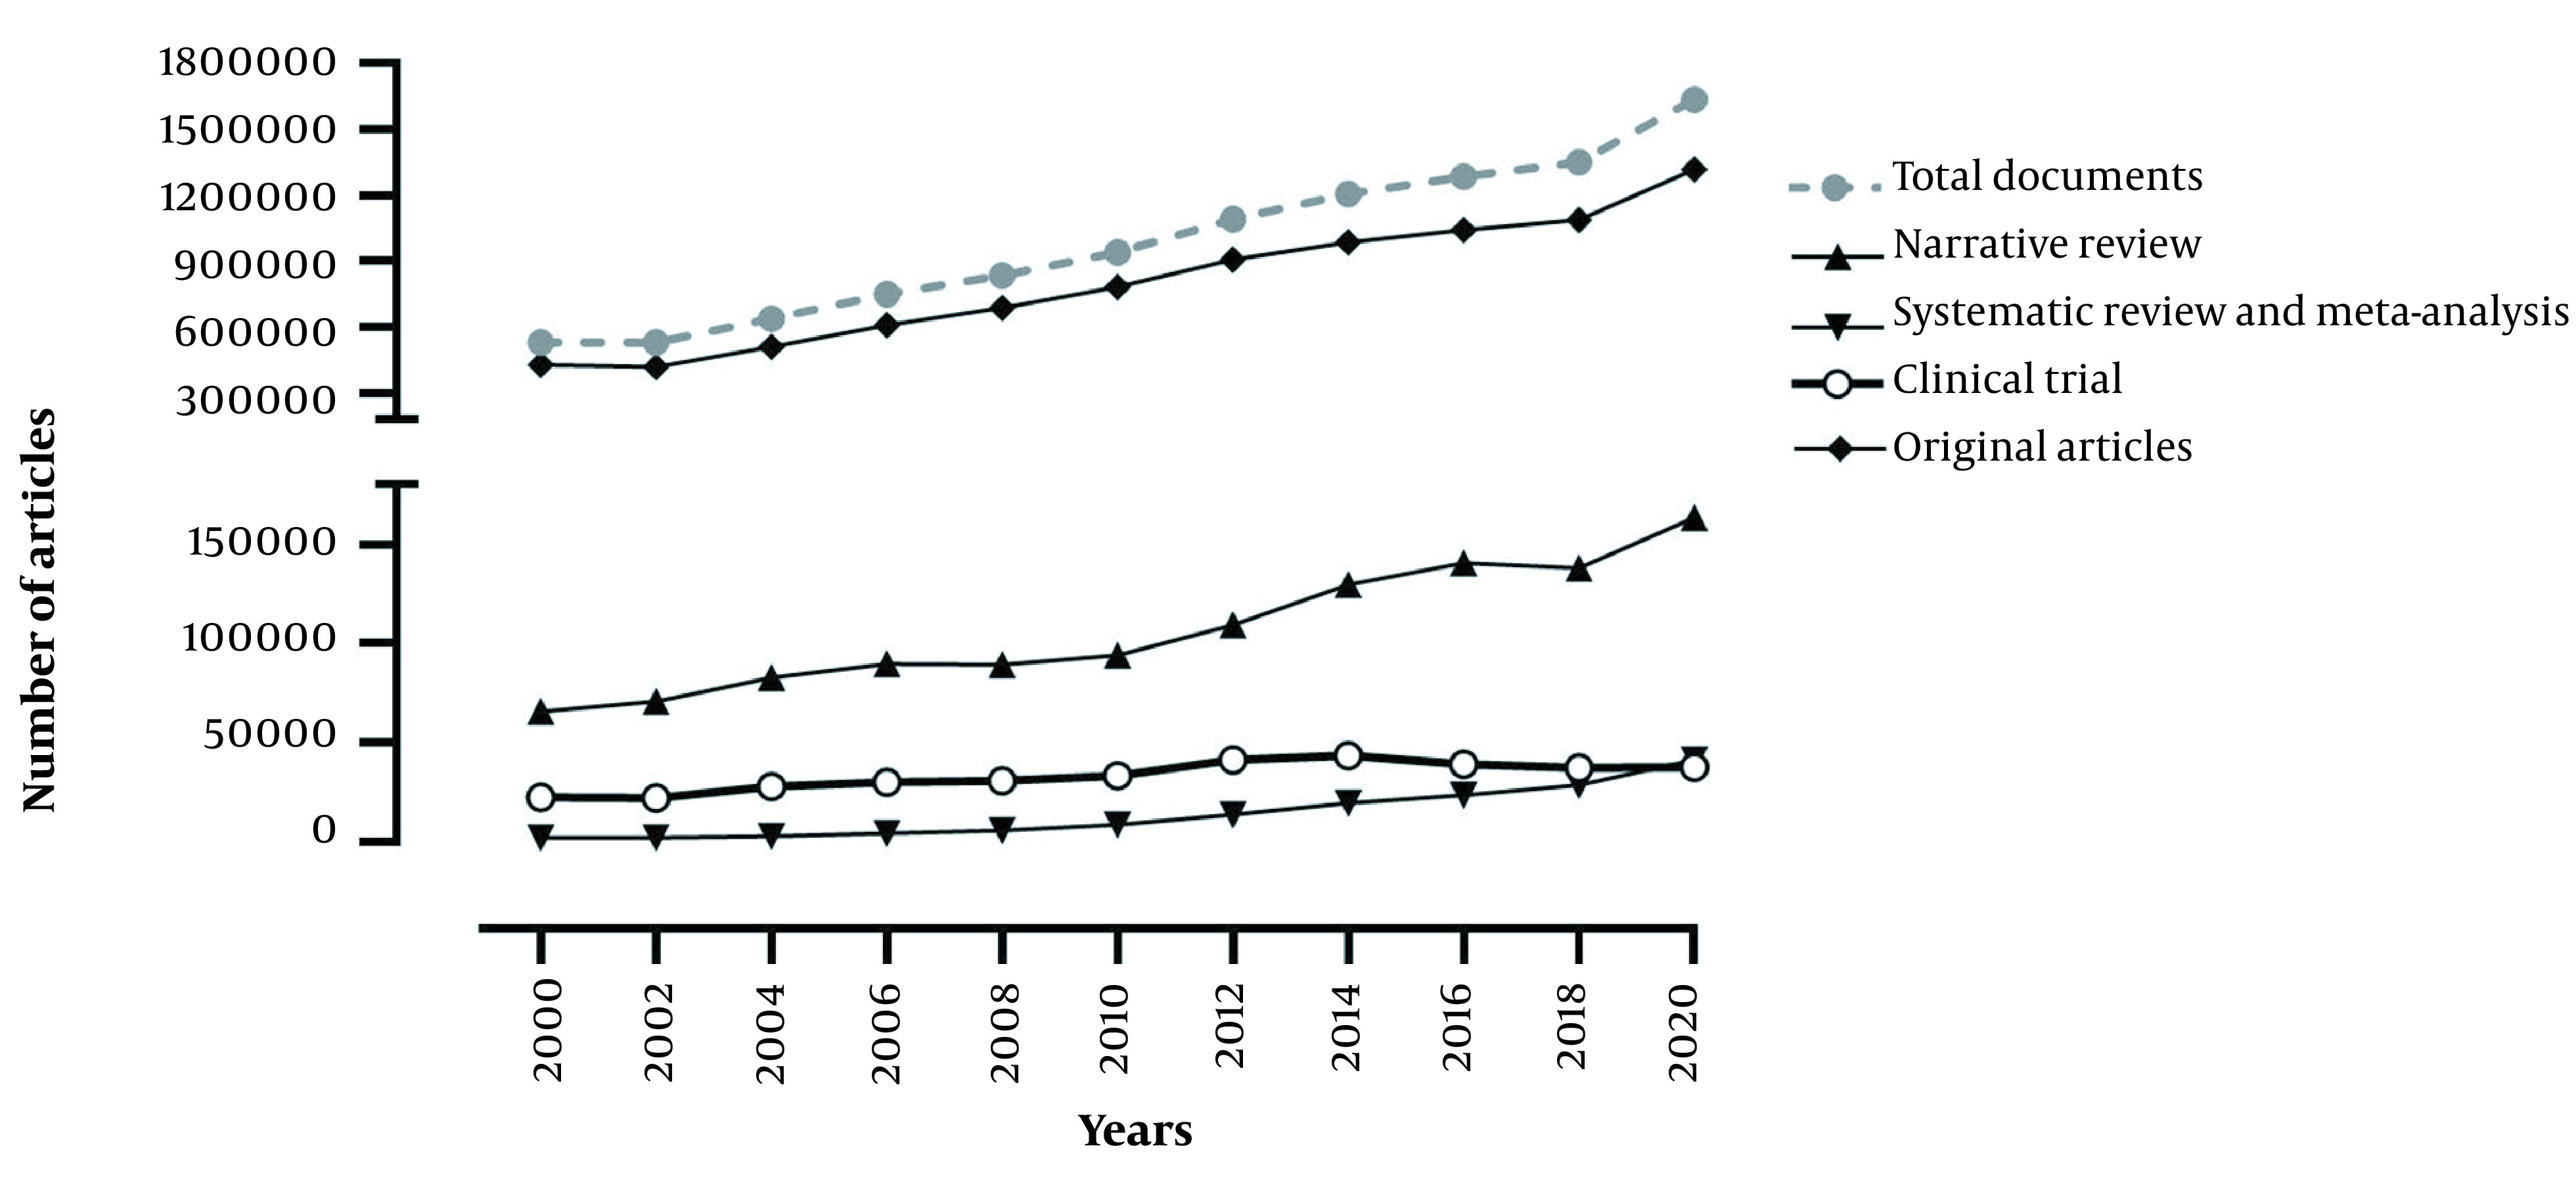
\includegraphics[width=1\linewidth]{images/increase_in_publications.jpg}
    \caption{Increasing publications over that past two decades \cite{ghasemi_scientific_2022}.}
    \label{fig:increasing_publications_over_time}
\end{figure}

The publication rate of systematic reviews in medicine has surged exponentially in recent decades, a trend reflecting their growing centrality to evidence-based practice. Between 1986 and 2015, PubMed indexed a 2,728\% increase in articles labelled as systematic reviews, far outpacing the 153\% rise in other publications during the same period \cite{ioannidis_mass_2016}. This expansion underscores a growing need for consolidated, high-quality evidence to address diverse clinical questions, especially as the volume of primary research increases. For instance, the number of clinical trials—a key source of evidence—doubled between 2001 and 2020, while peer-reviewed journals nearly tripled \cite{ghasemi_scientific_2022}; see Figure \ref{fig:increasing_publications_over_time}). Methodological advances, such as PRISMA guidelines and GRADE frameworks, have strengthened systematic review rigour, enabling them to shape clinical guidelines, inform policy, and even synthesise overlapping evidence through umbrella reviews. Cochrane exemplifies this impact: its 9,000+ systematic reviews, accessed over 17.5 million times by 2023, underscore its global reach and influence, reflected in a journal impact factor of 8.8\footnote{https://www.cochrane.org/about-us/scientific-strategy}.


\subsection{The process}

% Brief overview of the Cochrane Review process and its characteristics.
Although no single universally correct method exists for conducting a medical systematic review, with various approaches available (e.g., Joanna Briggs Institute review \cite{santos_joanna_2018}, Network Meta-Analysis \cite{bafeta_reporting_2014}, or meta-analysis\cite{moher_improving_1999}) \cite{munn_what_2018}, the Cochrane Review is a commonly used process \cite{cipriani_what_2011}. The Cochrane Review framework is particularly relevant to this PhD because each step is meticulously documented, enabling potential automation.


\begin{itemize}
    \item {\bf{Standardised Methodology:}} systematic reviews often use a PICO format (Patient, Intervention, Comparison, Outcome). All reviews follow strict guidelines in the Cochrane Handbook, ensuring consistency. This process minimises bias through methods like dual study selection and data extraction by multiple authors.
    \item {\bf{Mandatory Protocol Registration:}} Cochrane Reviews require protocol registration before the review commences, reducing bias from post-hoc changes \cite{cumpston_chapter_2024}.
    \item {\bf{Regular Updates:}} Cochrane systematic reviews are updated periodically to reflect new evidence.
    \item {\bf{GRADE framework for evidence certainty:}} Uses a system (high, moderate, low, very low) to rate the certainty of evidence in the summary of findings table \cite{guyatt_grade_2008}.
\end{itemize}


% Focus on the search process within Cochrane reviews.

\gls*{ir} — often led by medical and healthcare librarians or information specialists (\gls*{ir} specialists) — plays a vital role in producing high-quality Cochrane Reviews. Their \gls*{ir} expertise ensures the comprehensiveness and rigour of the systematic review process. Extensive research confirms the positive impact of \gls*{ir} specialists' involvement in systematic reviews, highlighting their contributions to both the search process \cite{le_benchmarking_2023, brunskill_case_2022, schvaneveldt_assessing_2021} and overall search quality \cite{giroudon_qualite_2023, pawliuk_librarian_2024, ramirez_adherence_2022}. Collaboration between \gls*{ir} specialists and review authors spans the early planning stages to the final write-up and subsequent updates.

\gls*{ir} specialists perform a wide range of tasks, including:

\begin{itemize}
\item {\bf{Source Selection:}} Advising authors on selecting appropriate databases and other sources tailored to the specific review topic.
\item {\bf{Search Strategy Development:}} Designing or guiding the development of comprehensive and sensitive search strategies for major bibliographic databases and trial registers.
\item {\bf{Search Execution:}} Running searches in databases and trial registers accessible to the \gls*{ir} specialist.
\item {\bf{Results Management:}} Saving, collating, and sharing search results with authors in suitable formats, including de-duplicating records.
\item {\bf{Protocol and Review Development:}} Drafting or assisting in drafting the search methods sections of Cochrane protocols, reviews, and updates.
\item {\bf{Methodological Compliance:}} Ensuring that Cochrane protocols, reviews, and updates adhere to the Methodological Expectations of Cochrane Intervention Reviews (MECIR) related to searching activities.
\item {\bf{Translation Organisation:}} Facilitating the translation or data extraction of studies reported in languages other than English, enabling assessment of these reports for inclusion or exclusion.
\item {\bf{Document Retrieval:}} Obtaining copies of trial reports for review teams when needed.
\item {\bf{Formatting and Style:}} Checking and formatting the references to included and excluded studies according to the Cochrane Style Manual.
\end{itemize}

Because \gls*{ir} specialists undertake a wide range of tasks, understanding the structure of the systematic review process is crucial. The systematic review process consists of five phases, as shown in Table \ref{tab:stages_of_systematic review}. Because \gls*{ir} specialists' expertise is essential for Stage 2 (Identifying relevant work), this PhD research focuses on optimising processes within this stage. This stage can be further granularised into several substages, many of which directly involve the tasks outlined above:

\begin{itemize}
\item {\bf{Inclusion/exclusion criteria generation:}} Defining the precise criteria for including or excluding studies, supported by \gls*{ir} specialist guidance on source selection and search strategy development.
\item {\bf{Search Strategy Development:}} Creating the detailed search algorithms used to query databases (a core \gls*{ir} specialist responsibility).
\item {\bf{Database Searching:}} Implementing the search strategy across various databases and trial registers (conducted by \gls*{ir} specialists).
\item {\bf{Protocol Writing:}} Documenting the search methodology in detail, with \gls*{ir} specialists contributing the search methods section.
\item {\bf{Title and Abstract Screening:}} Initially assessing study relevance based on titles and abstracts, facilitated by \gls*{ir} specialist results management and de-duplication.
\item {\bf{Full-Text Download and Screening:}} Obtaining and reviewing the full text of potentially relevant studies supported by \gls*{ir} specialist document retrieval.
\item {\bf{Manual Search:}} Supplementing database searches with manual searching of relevant journals, conference proceedings, and other sources, often guided by \gls*{ir} specialists.
\end{itemize}



\begin{table*}[t]
\centering
\small
\begin{tabular}{|c|p{0.85\textwidth}|}
\hline
\textbf{Stage} & \textbf{Purpose} \\
\hline
1 & \textbf{Framing questions for a review:} The research question is structured and explicitly formulated. \\\hline
2 & \textbf{Identifying relevant work:} A wide range of databases are searched to identify research to be included. Potential research is first identified, screened, eligibility checked, and then a decision is made on the inclusion of that research \cite{tawfik_step_2019}. \\\hline
3 & \textbf{Assessing the quality of studies:} Research is tested for quality, such as minimum research design, and subjected to higher quality assessment checks, including tests for research heterogeneity. \\\hline
4 & \textbf{Summarizing the evidence:} Data synthesis occurs with tabulation of study characteristics and quality. Statistical testing is performed at this stage. \\\hline
5 & \textbf{Interpreting the findings:} Any issues highlighted in the previous steps should be addressed. Generate recommendations guided by reference to the strength of the evidence. \\
\hline
\end{tabular}
\caption{Stages of a Systematic Review.}
\label{tab:stages_of_systematic review}
\end{table*}



% Focus on the title and abstract screening substage.
This PhD research focuses on the Title and Abstract screening substage of the `Identifying Relevant Work' phase, a critical process often visualised using the PRISMA flow diagram (Figure \ref{fig:prisma_flow}). This stage alone is estimated  to account for 10-20\% of the time it takes to plan and conduct a systematic review \cite{haddaway_predicting_2019}.

\begin{figure}
    \centering
    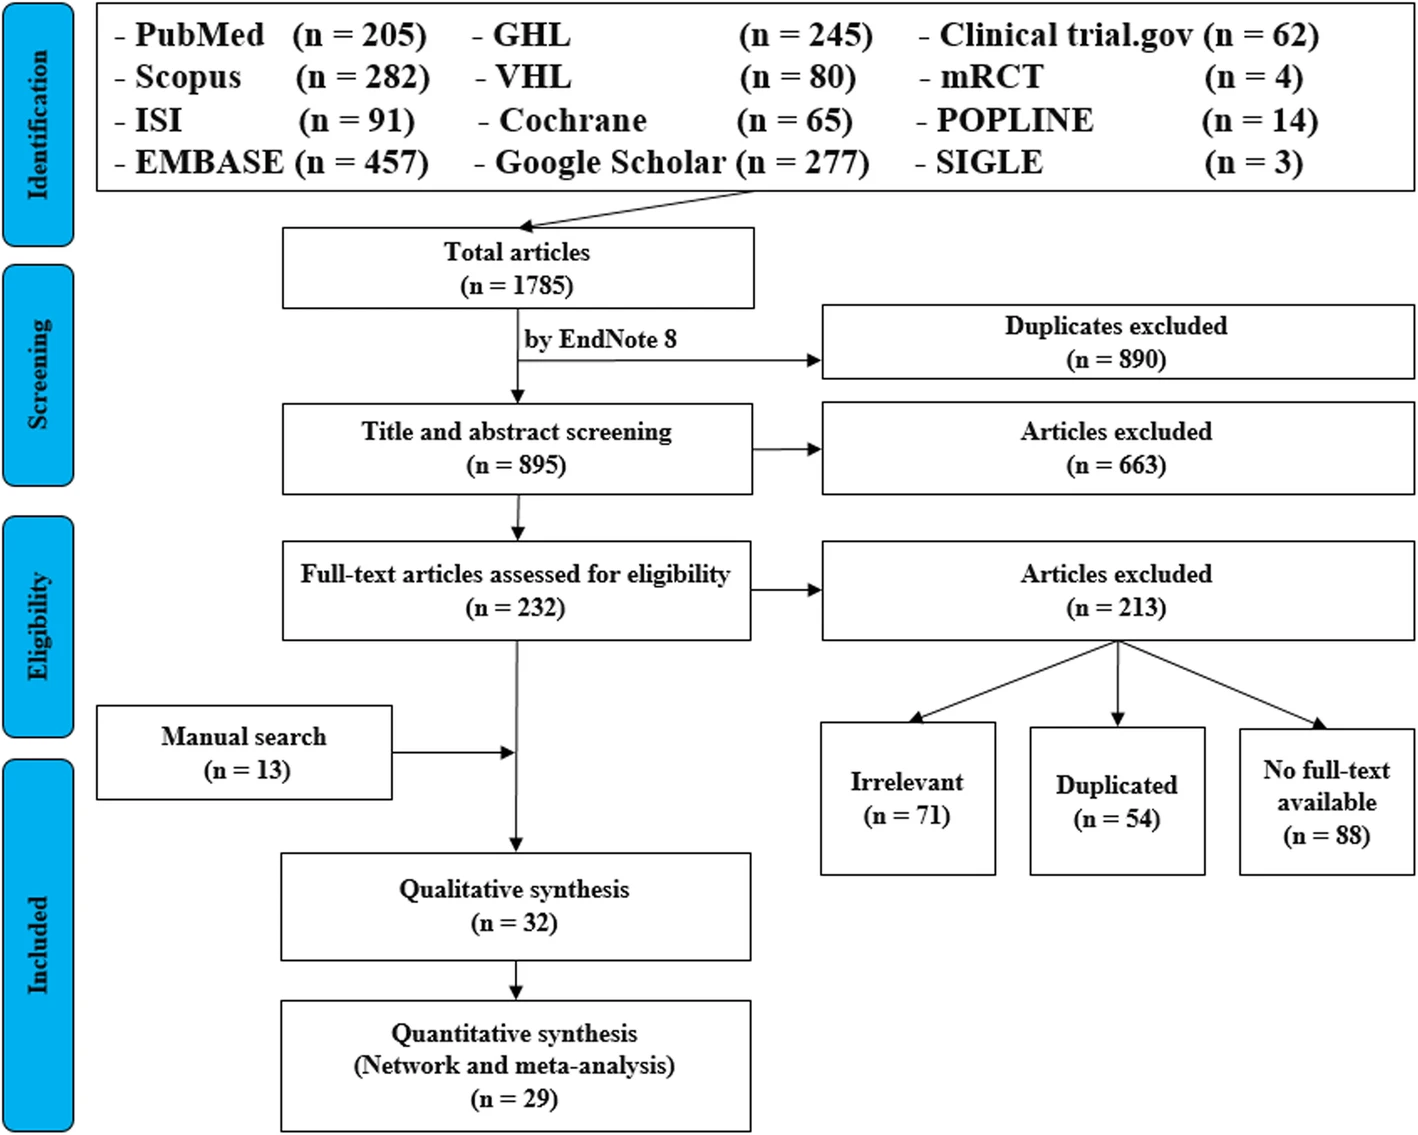
\includegraphics[width=0.5\linewidth]{Confirmation Review//images/prisma_flow.png}
    \caption{PRISMA flow diagram for a simulated Cochrane systematic review \cite{tawfik_protocol_2020}. Note the different substages of the identification of relevant work in blue.}
    \label{fig:prisma_flow}
\end{figure}

The identification stage compiles all potential studies from searched databases into a large dataset $T$ of studies that may or may not be relevant to the systematic review. Screening further refines this pool by removing duplicates and assessing titles and abstracts to reduce the number of full-text articles requiring assessment in the eligibility substage. Traditionally, 2-3 reviewers manually evaluate titles and abstracts to determine whether each study should be included or excluded based on predetermined criteria. At this stage, studies are typically categorised as relevant (related to the systematic review) or not relevant (unrelated to the systematic review).

% Research within the title and abstract screening substage

Best practices have been outlined to increase consistency and reduce bias in the title and abstract screening phase \cite{polanin_best_2019}. At the start of this stage, using an abstract screening tool with clear, concise questions and conducting training sessions where screeners learn and pilot test the screening process using 20-30 abstracts is recommended to ensure intercoder agreement. During the screening phase, teams should hold weekly meetings, avoid changes to the screening tool, use text-mining, employ independent double-screening of each work, and immediately reconcile disputes. After the screening phase, analysing the process itself for validity is recommended.

Research on title and abstract screening reveals crucial elements for successful outcomes and strongly supports using both the title \emph{and} abstract. For instance, recent work comparing title-only (Ti/O) versus title-plus-abstract (Ti+Ab) screening found that Ti+Ab achieved significantly higher sensitivity (94.7\% vs. 57.9\%) by capturing studies with ambiguous titles but relevant abstract content. At the same time, Ti/O risked excluding 42.1\% of eligible studies due to insufficient title clarity \cite{teo_title-plus-abstract_2023}. Another study showed that adopting a Title-First screening approach (rejecting a study based on the title, followed by abstract assessment for inclusion) reduced workload compared to a title-and-abstract approach, with no reduction in recall of relevant research \cite{mateen_titles_2013}. The use of non-experts (medical students) as a feasible alternative to experts when undertaking citation screening was demonstrated in the TASER study \cite{ng_title_2014}.


\subsection{Challenges}

% Resource usage
The main challenges fall into three categories: resource use, consistency, and bias. The title and abstract screening stage often involves hundreds or thousands of potentially relevant studies, each requiring assessment by at least one, ideally two, trained reviewers. This scale is not trivial. Estimates suggest that a proficient information specialist can screen between 0.133 and 2.88 abstracts per minute \cite{shemilt_use_2016,giummarra_evaluation_2020,felizardo_visual_2013}; consequently, screening a large volume of abstracts is a significant undertaking. This task's sheer scale demands considerable time from expert reviewers, whose expertise is costly and scarce, thus increasing the financial burden of conducting systematic reviews

Furthermore, attempts to mitigate costs by reducing screening requirements, such as employing a single reviewer, substantially compromise the recall of relevant studies. \gls*{rcts} using the Cochrane Crowd platform demonstrated that single-reviewer approaches could miss up to 13\% of relevant studies, whereas a dual-reviewer approach missed only 3\% \cite{gartlehner_single-reviewer_2020}. Similar findings have been reported in other studies, indicating that even experienced reviewers, when working in isolation, consistently missed more relevant references \cite{waffenschmidt_single_2019}. Because minimising the risk of excluding pertinent evidence is crucial, dual screening is considered indispensable despite the associated resource implications.

The temporal demands of systematic reviews are also substantial, with an average completion time of 67.3 weeks \cite{borah_analysis_2017}. The screening phase alone can prolong the timeline by several months. While the precise number of abstracts screened per review is not uniformly documented, surveys of established systematic reviews report a median of 555 abstracts, spanning from 232 to 9,648 \cite{nama_successful_2021}. In one analysis of 14 systematic reviews, 19,334 abstracts were screened, yielding only 3.1\% (605) relevant studies \cite{nama_successful_2021}. At such scales, reviewer fatigue poses a legitimate concern, as prolonged engagement in tedious screening tasks can diminish vigilance and compromise the accuracy of the review process.


% % Consistency 
% Consistently applying inclusion and exclusion criteria across all studies poses a persistent challenge, with inter-coder discrepancies common, even when two reviewers evaluate the same abstracts. This is particularly true for studies in a ``grey area" that require nuanced judgment for inclusion or exclusion. Resolving these discrepancies typically requires discussion between reviewers or consultation with a third, adding roughly 5 minutes per conflict \cite{shemilt_use_2016}. With thousands of abstracts, this resolution process significantly increases resource and time demands. Moreover, inherent variability within review teams—differing expertise, subjective interpretations, and individual biases—fosters inconsistencies. Although rigorous pilot testing and ongoing calibration exercises help, consistently applying criteria remains challenging, especially over extended screening periods with numerous abstracts.

% % Bias
% Bias in title and abstract screening occurs when certain studies are systematically favoured or excluded. Several factors contribute to this risk: 
% \begin{itemize} 
% \item \textbf{Single-reviewer bias:} As previously discussed, single-reviewer approaches miss more eligible studies, potentially reducing the comprehensiveness of the final evidence base.
% \item \textbf{User fatigue:} Extended screening periods can cause ``attention drift", leading reviewers to exclude relevant studies inadvertently.
% \item \textbf{Prior knowledge and expectations:} Reviewers with pre-existing knowledge may unconsciously favour studies aligning with their beliefs or published in well-regarded journals. Conversely, they may dismiss studies they deem less relevant, introducing selection bias.
% \end{itemize}

% % Bias Ctd
% Another source of bias is assuming humans always label documents correctly. Wang et al. report error rates as high as 10.76\% during abstract screening \cite{wang_error_2020}. While strategies like dual-review and reporting inter-coder agreements help, they do not guarantee error elimination.



\end{document}
